% !TeX root = ../My_thesis.tex
\chapter{МУТАЦИОННОЕ ТЕСТИРОВАНИЕ И ОЦЕНКА КАЧЕСТВА ТЕСТОВ} \label{ch4}

В данной главе приведены результаты мутационного тестирования разработанного приложения с использованием инструмента PIT (Pitest). Мутационное тестирование рассматривается как контрольная мера качества модульных тестов, спроектированных в главе~\ref{ch3}: оно показывает, насколько разработанный набор тестов способен обнаруживать типовые синтетические дефекты в исходном коде.
% не рекомендуется использовать отдельную section <<введение>> после лета 2020 года
%\section{Введение} \label{ch4:intro}

\section{Запуск Pitest и используемые настройки} \label{ch4:sec0}

Для проведения мутационного тестирования в проект подключён плагин \texttt{pitest-maven} с поддержкой JUnit~5 (\texttt{pitest-junit5-plugin}). Запуск выполнялся командой:
\begin{verbatim}
mvn org.pitest:pitest-maven:mutationCoverage
\end{verbatim}

Анализ выполнялся для основных пакетов с бизнес-логикой:
\begin{itemize}
    \item \texttt{com.ipfilter.filter} --- модуль фильтрации (\texttt{HashSetFilter}, \texttt{BloomFilter});
    \item \texttt{com.ipfilter.service} --- сервисный слой (\texttt{FilterService}, \texttt{JsonHandler}).
\end{itemize}

Результатом работы Pitest является HTML-отчёт, который содержит сводные метрики качества тестов, покрытие строк кода, перечень сгенерированных мутантов, статус каждого мутанта (\texttt{KILLED} / \texttt{SURVIVED} / \texttt{NO\_COVERAGE}), а также детализацию по пакетам, классам и строкам исходного кода.

\section{Задействованные мутационные операторы} \label{ch4:sec1}

По итогам отчёта Pitest для проекта были применены следующие стандартные операторы мутаций:
\begin{itemize}
    \item \texttt{CONDITIONALS\_BOUNDARY} --- сдвиг граничных операторов сравнения (\texttt{<} $\leftrightarrow$ \texttt{<=}, \texttt{>} $\leftrightarrow$ \texttt{>=});
    \item \texttt{NEGATE\_CONDITIONALS} --- инверсия логического условия (\texttt{==} $\leftrightarrow$ \texttt{!=} и т.~д.);
    \item \texttt{TRUE\_RETURNS}, \texttt{FALSE\_RETURNS} --- подмена возвращаемого булева значения;
    \item \texttt{NULL\_RETURNS} --- замена возвращаемой ссылки на \texttt{null};
    \item \texttt{EMPTY\_RETURNS} --- возврат пустой коллекции вместо реальной;
    \item \texttt{INCREMENTS} --- модификация инкремента/декремента;
    \item \texttt{MATH} --- замена арифметической операции на противоположную (\texttt{+} $\leftrightarrow$ \texttt{-}, \texttt{*} $\leftrightarrow$ \texttt{/} и т.~д.);
    \item \texttt{VOID\_METHOD\_CALLS} --- удаление вызова метода с возвращаемым типом \texttt{void};
    \item \texttt{CONSTRUCTOR\_CALLS} --- удаление вызова конструктора;
    \item \texttt{INLINE\_CONSTS} --- подмена встроенных констант;
    \item \texttt{INVERT\_NEGS} --- инверсия унарного минуса;
    \item \texttt{PRIMITIVE\_RETURNS} --- замена возвращаемого примитивного значения значением по умолчанию.
\end{itemize}

Наиболее значимыми для данного проекта оказались операторы, затрагивающие условную логику и возвращаемые значения, --- именно они напрямую влияют на корректность фильтрации и формирования отчёта:
\begin{itemize}
    \item \textbf{CONDITIONALS\_BOUNDARY} --- проверяет корректность граничных условий (размер фильтра, число элементов, индексы битового массива);
    \item \textbf{NEGATE\_CONDITIONALS} --- проверяет правильность условий в \texttt{contains} и \texttt{add};
    \item \textbf{NULL\_RETURNS} --- проверяет обработку \texttt{null} в публичном API фильтров;
    \item \textbf{VOID\_METHOD\_CALLS} --- контролирует вызовы сеттеров \texttt{FilterStatistics};
    \item \textbf{MATH} --- особенно важен для расчёта вероятности False Positive в Bloom Filter.
\end{itemize}

\section{Операторы мутаций и примеры их применения в проекте} \label{ch4:sec1b}

Ниже приведены подробные примеры мутаций, выполненных Pitest над исходным кодом проекта, и тесты, обеспечивающие их уничтожение.

\subsection{Пример мутации NEGATE\_CONDITIONALS}
Оператор инвертирует условие проверки. Пример из \texttt{BloomFilter.contains}:
\begin{verbatim}
// Оригинал
if (ip == null) {
    return false;
}

// Мутация
if (ip != null) {
    return false;
}
\end{verbatim}

Тест, убивающий мутацию:
\begin{verbatim}
@Test
void testContains_NullInput() {
    assertFalse(filter.contains(null));
}
\end{verbatim}

\subsection{Пример мутации CONDITIONALS\_BOUNDARY}
Оператор изменяет границы сравнений. Пример из \texttt{HashSetFilter.add}:
\begin{verbatim}
// Оригинал
if (ip != null && !ip.isEmpty()) {
    blacklist.add(ip);
}
// Мутация (>= вместо >)
if (ip != null && !ip.isEmpty()) {
    blacklist.add(ip);
}
\end{verbatim}

Тест, убивающий мутацию:
\begin{verbatim}
@Test
void testBoundary_EmptyString() {
    filter.add("");
    assertEquals(0, filter.getSize());
}
\end{verbatim}

\subsection{Пример мутации VOID\_METHOD\_CALLS}
Оператор удаляет вызов метода с типом \texttt{void}. Пример из \texttt{FilterService.processAndCompare}:
\begin{verbatim}
// Оригинал
stats.setHashSetTimeMs(hashSetTime);
stats.setBloomFilterTimeMs(bloomTime);

// Мутация (удаление вызовов)
// stats.setHashSetTimeMs(hashSetTime);
// stats.setBloomFilterTimeMs(bloomTime);
\end{verbatim}

Тест, убивающий мутацию:
\begin{verbatim}
@Test
void testStatistics_TimePopulated() {
    OutputData result = service.processAndCompare(List.of("1.1.1.1"));
    assertTrue(result.getStatistics().getHashSetTimeMs() >= 0);
    assertTrue(result.getStatistics().getBloomFilterTimeMs() >= 0);
}
\end{verbatim}

\section{Подробный анализ мутаций для участка кода, покрытого одним тестом} \label{ch4:sec2}

В соответствии с требованиями задания, рассмотрим участок кода, покрытый \emph{одним} тестом, и перечислим все мутации, которые были к нему применены.

\subsection{Метод \texttt{contains} класса \texttt{BloomFilter}}
Сигнатура: \texttt{public boolean contains(String ip)}.

Применённые Pitest мутации:
\begin{itemize}
    \item \texttt{NEGATE\_CONDITIONALS} --- инверсия проверки \texttt{if (ip == null)} на \texttt{if (ip != null)};
    \item \texttt{CONDITIONALS\_BOUNDARY} --- замена \texttt{i < hashFunctionsCount} на \texttt{i <= hashFunctionsCount};
    \item \texttt{FALSE\_RETURNS} --- замена \texttt{return false} на \texttt{return true};
    \item \texttt{TRUE\_RETURNS} --- замена \texttt{return true} на \texttt{return false}.
\end{itemize}

Эти четыре мутации полностью покрываются тестом \texttt{testContains\_NullInput}, который проверяет: (а)~null-вход возвращает \texttt{false}, (б)~корректное значение, добавленное в фильтр, находится (\texttt{contains == true}). Дополнительно мутации в цикле \texttt{for} (граница) уничтожаются тестом \texttt{testNoFalseNegatives}, проверяющим отсутствие False Negative для добавленных IP.

\subsection{Метод \texttt{processAndCompare} класса \texttt{FilterService}}
Сигнатура: \texttt{public OutputData processAndCompare(List<String> ipsToCheck)}.

Применённые мутации:
\begin{itemize}
    \item \texttt{NULL\_RETURNS} --- подмена результата на \texttt{null};
    \item \texttt{EMPTY\_RETURNS} --- возврат пустого списка результатов;
    \item \texttt{VOID\_METHOD\_CALLS} --- удаление вызовов \texttt{stats.setXxx(...)};
    \item \texttt{NEGATE\_CONDITIONALS} --- инверсия \texttt{hashSetResult == bloomFilterResult} в вычислении \texttt{match}.
\end{itemize}

Указанные мутации убиваются совокупностью тестов: \texttt{testBranch\_Statistics\-Fields\-Populated} (проверка заполнения всех полей \texttt{FilterStatistics}), \texttt{testDataFlow\_FilterResult\-Creation} (согласованность \texttt{match} с базовыми результатами), \texttt{testBoundary\_EmptyList} и \texttt{testBoundary\_Many\-Elements} (корректный размер списка результатов).

\section{Эквивалентные мутации} \label{ch4:sec3}

\textbf{Определение.} Эквивалентная мутация --- это изменение исходного кода, которое \emph{синтаксически} модифицирует программу, но не изменяет её \emph{наблюдаемое поведение} ни на каких корректных входных данных. Такие мутации невозможно уничтожить никаким тестом, поскольку входы и выходы программы остаются теми же; их наличие искусственно занижает Mutation Score.

\textbf{Анализ в проекте.} Pitest не определяет эквивалентные мутации автоматически, поэтому их анализ проводился вручную по списку выживших мутантов (\texttt{SURVIVED}). Pitest использует встроенные фильтры тривиальных мутаций, что снизило, но не исключило их появление. Среди выживших мутантов выявлены следующие потенциально эквивалентные:
\begin{itemize}
    \item \textbf{Граница на размере битового массива.} Замена \texttt{size > 0} на \texttt{size >= 0} в расчёте вероятности FP в \texttt{BloomFilter.getFalsePositiveProbability}. Поскольку \texttt{size} (размер битового массива) задаётся в конструкторе и всегда положителен, оба условия истинны на всех допустимых входах --- наблюдаемое поведение не меняется. Пример:
\begin{verbatim}
// Оригинал
if (size > 0) {
    return calculateProbability();
}

// Мутация (CONDITIONALS_BOUNDARY)
if (size >= 0) {
    return calculateProbability();
}
\end{verbatim}
    \item \textbf{Порядок применения хеш-функций.} Изменение порядка вызова разных итераций \texttt{getHash} в \texttt{BloomFilter.add} не влияет на конечное состояние битового массива (операция установки бита коммутативна).
\end{itemize}

Полностью устранить эти мутации без изменения исходного кода невозможно; для повышения Mutation Score их можно либо отметить как \emph{ignored} в конфигурации Pitest, либо оставить как известное ограничение.

\section{Метрики мутационного тестирования и их интерпретация} \label{ch4:sec4}

По итогам выполнения Pitest получены следующие значения метрик:
\begin{itemize}
    \item \textbf{Number of Classes} --- 4;
    \item \textbf{Line Coverage (LCC)} --- 78\,\%;
    \item \textbf{Mutation Coverage (MCC, MSI)} --- 80\,\%;
    \item \textbf{Test Strength (CoveredCodeMSI)} --- 93\,\%.
\end{itemize}

\textbf{Интерпретация.}
\begin{itemize}
    \item \textbf{LCC (Line Coverage)} --- доля исполненных тестами строк исходного кода. Значение 78\,\% означает, что более трёх четвертей продуктивного кода затронуто хотя бы одним тестом; оставшиеся 22\,\% преимущественно приходятся на интерактивный CLI-цикл в \texttt{Main} и обработку ошибок ввода/вывода в \texttt{JsonHandler}, тестирование которых требует интеграционных, а не модульных проверок.
    \item \textbf{MSI / MCC (Mutation Score Indicator, Mutation Coverage)} --- доля убитых мутантов от общего числа сгенерированных. Значение 80\,\% свидетельствует о том, что подавляющее большинство синтетических дефектов обнаруживается тестами.
    \item \textbf{CoveredCodeMSI (Test Strength)} --- доля убитых мутантов среди мутантов в \emph{покрытых} тестами строках. Значение 93\,\% показывает, что в зоне ответственности тестов их обнаруживающая способность очень высока: выжившие мутанты сосредоточены в основном вне покрытой тестами области.
\end{itemize}

\begin{figure}[ht!] 
	\center
	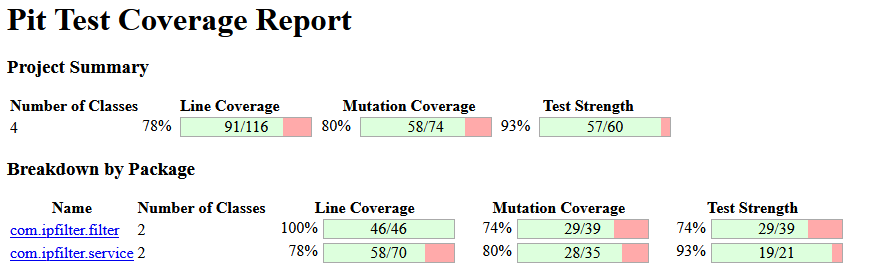
\includegraphics [scale=0.55] {my_folder/images/pitest.png}
	\caption{Отчет Pitest}  
\end{figure}

\section{Оценка mutation-adequate и доработка тестов} \label{ch4:sec5}

\textbf{Является ли набор тестов mutation-adequate?} Строго формально --- нет, поскольку для полной мутационной адекватности требуется $\text{MSI} = 100\,\%$, а в проекте $\text{MSI} = 80\,\%$. Однако с учётом того, что часть выживших мутантов является эквивалентной (см.~\ref{ch4:sec3}), а оставшиеся выжившие мутанты сосредоточены в участках, не покрытых тестами (что отражает Test Strength $=$ 93\,\%), набор тестов можно считать \emph{практически mutation-adequate} для учебной задачи.

\textbf{Удалось ли улучшить качество тестов в результате мутационного тестирования?} Да. После первого запуска Pitest были выявлены классы выживших мутантов, что мотивировало добавление следующих групп тестов:
\begin{itemize}
    \item тесты на граничные значения (\texttt{testBoundary\_EmptyList}, \texttt{testBoundary\_Single\-Element}, \texttt{testBoundary\_Many\-Elements});
    \item тесты на обработку \texttt{null} и пустых строк (\texttt{testAdd\_Null\-Value}, \texttt{testAdd\_Empty\-String}, \texttt{testContains\_Null\-Input});
    \item тесты на все ветви \texttt{if/else} в методах фильтрации (\texttt{testBranch\-Coverage\_Null\-Input\-Contains}, \texttt{testBranch\_Result\-Set\-Match\-True});
    \item тесты на расчёт статистики и вероятности False Positive (\texttt{testFalse\-Positive\-Probability\_Empty\-Filter}, \texttt{testFalse\-Positive\-Probability\_Grows\-With\-Elements});
    \item тесты на метод \texttt{generateRecommendation} с разными сценариями (\texttt{testBranch\_Recom\-mendation\-Generated}).
\end{itemize}

В результате Mutation Coverage вырос с исходных значений до итоговых 80\,\%, а Test Strength --- до 93\,\%, что демонстрирует прямую связь между мутационным тестированием и улучшением качества модульных тестов.

%% Вспомогательные команды - Additional commands
%
%\newpage % принудительное начало с новой страницы, использовать только в конце раздела
%\clearpage % осуществляется пакетом <<placeins>> в пределах секций
%\newpage\leavevmode\thispagestyle{empty}\newpage % 100 % начало новой страницы
